\documentclass[10pt,letterpaper,landscape]{article}
\usepackage[T1]{fontenc}
\usepackage{lmodern}
\usepackage{amsmath,amssymb}
\usepackage{graphicx}
\usepackage{booktabs}
\usepackage{geometry}
\usepackage{microtype}
\geometry{margin=0.55in}
\setlength{\parindent}{0pt}
\setlength{\parskip}{0.28em}
\pagestyle{plain}

\begin{document}
\begin{center}
{\Large\bfseries How the OCQKUDSIN Chebyshev coefficients grow}\\[0.2em]
{\small Square H$_4$; $\epsilon=0.5,\ 0.8,\ 1.2$; eight Lanczos states}
\end{center}

\textbf{What is plotted.}
For $H=\sum_\ell h_\ell P_\ell$, these three runs use the sine operator and
represent each normalized Lanczos state by
\[
\lambda=\sum_\ell|h_\ell|,\quad \bar H=H/\lambda,\quad
X_\epsilon=\sin(\epsilon\bar H),\quad
q_n=\sum_{m=0}^{n}c_{n,m}T_m(X_\epsilon)\Phi_0,
\quad n=0,\ldots,7.
\]
There are $n+1$ coefficients at iteration $n$. Each colored line below holds
the Chebyshev order $m$ fixed and follows $c_{n,m}$ as $n$ increases. A line
begins at $n=m$, when that coefficient first exists. The vertical axis is
$\log_{10}|c_{n,m}|$: a height of $4$ means $|c_{n,m}|\approx10^4$.
All plotted coefficients are real and positive.

\begin{center}
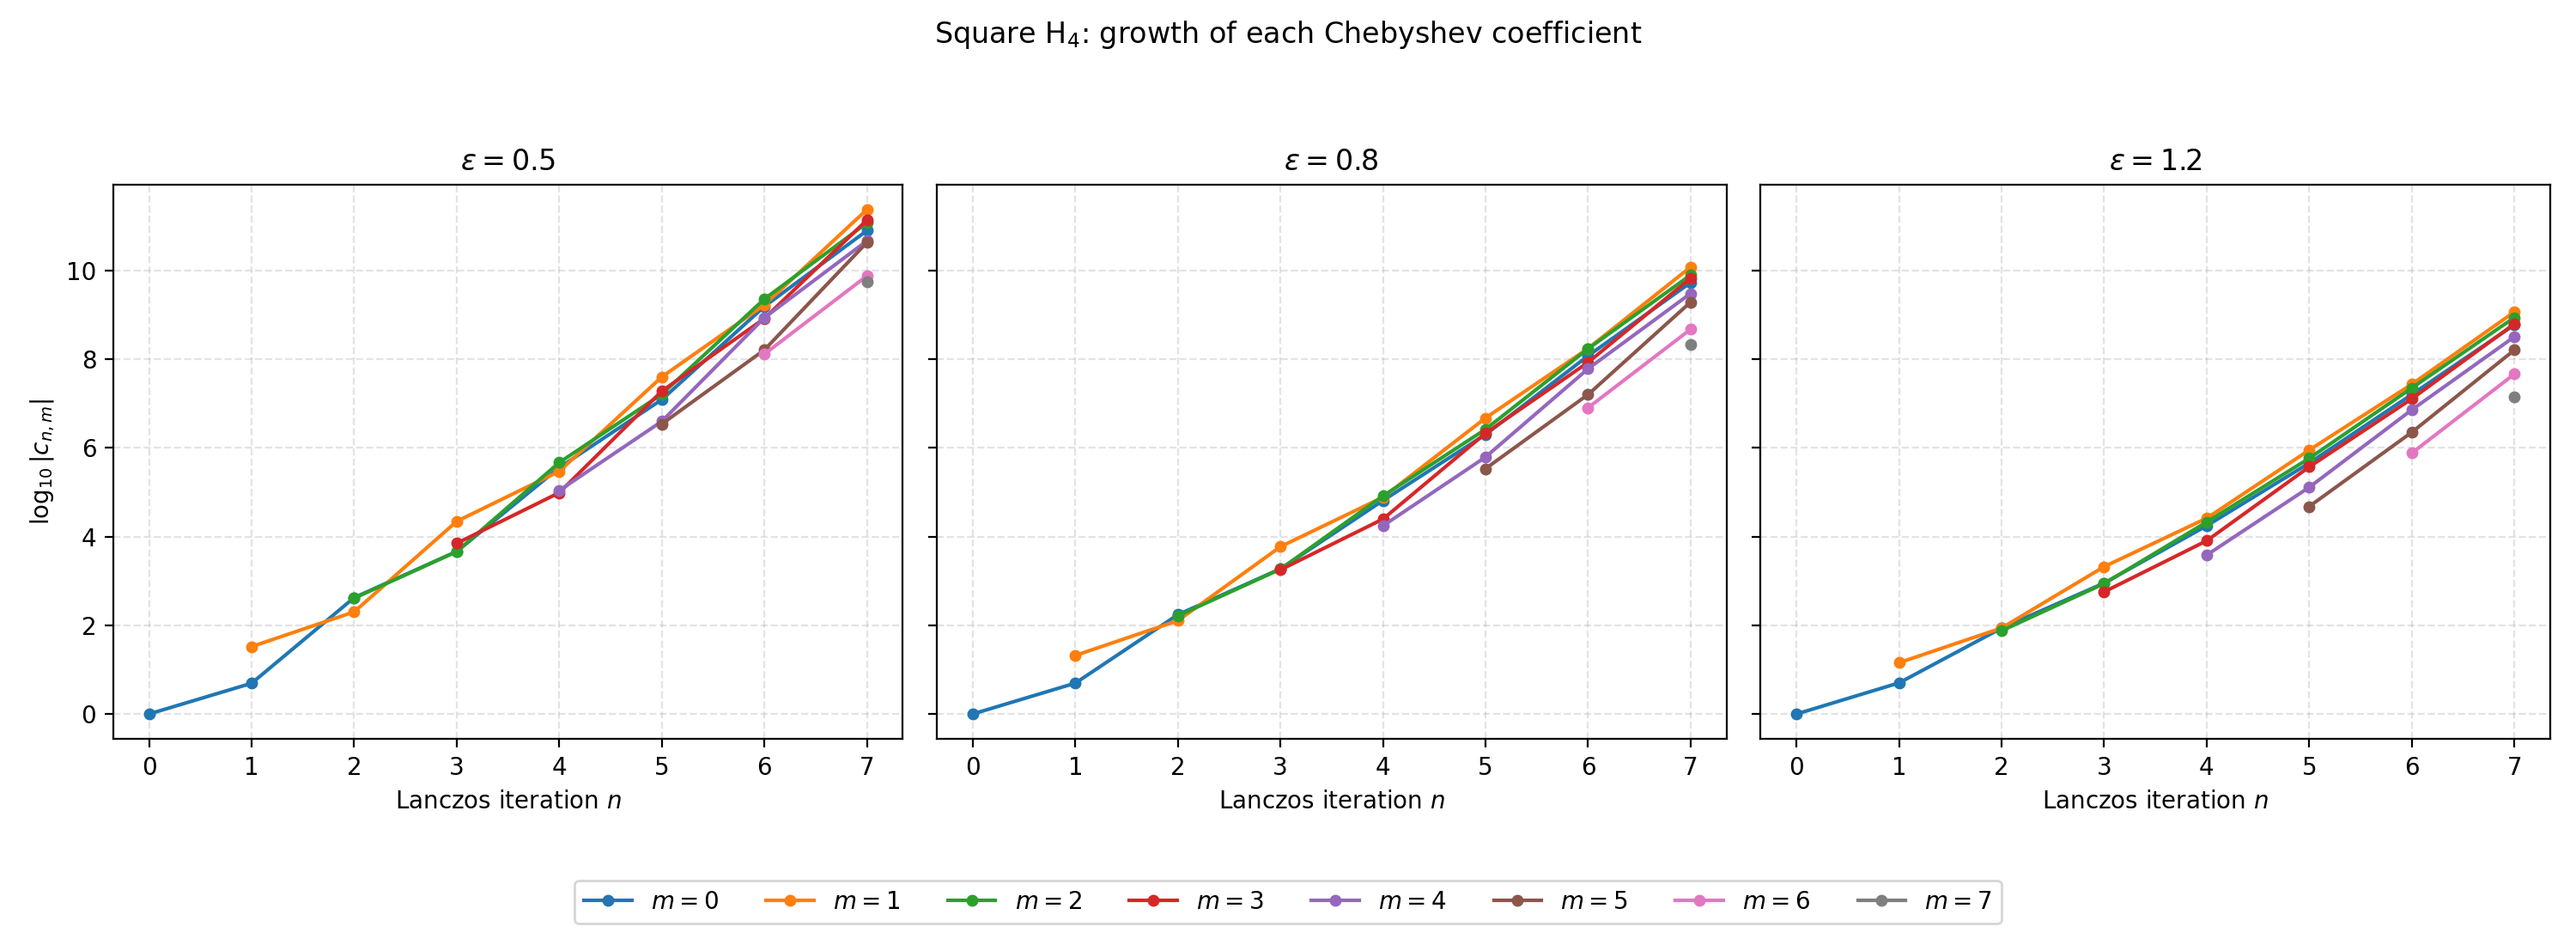
\includegraphics[width=0.90\linewidth]{output/ocqkudsin/chebyshev_coefficient_growth.png}
\end{center}

\vspace{-0.5em}
\textbf{Why they grow.}
The Lanczos recurrence and Chebyshev multiplication rule give
\[
\beta_{n+1}q_{n+1}=X_\epsilon q_n-\alpha_nq_n-\beta_nq_{n-1},\qquad
xT_0(x)=T_1(x),\quad
xT_m(x)=\tfrac12\bigl(T_{m-1}(x)+T_{m+1}(x)\bigr)\ (m\geq1).
\]
If $d_{n,m}$ is the coefficient of $T_m$ in $X_\epsilon q_n$, then
\[
c_{n+1,m}=\frac{d_{n,m}-\alpha_nc_{n,m}-\beta_nc_{n-1,m}}{\beta_{n+1}}.
\]
The small $\beta_{n+1}$ values repeatedly divide the coefficients. At
$\epsilon=0.5$, $\alpha_0=-0.14926558$ and $\beta_1=0.03029585$, so
\[
c_{1,0}=-\alpha_0/\beta_1=4.92693,\qquad
c_{1,1}=1/\beta_1=33.00782.
\]
The code evaluates each state with the Clenshaw recurrence, normalizes it,
and applies the same normalization factor to its coefficient row.

\newpage
\begin{center}
{\large\bfseries Measured growth and its interpretation}
\end{center}

\begin{minipage}[t]{0.46\linewidth}
\textbf{Largest coefficient at each iteration.}
These are $\max_m|c_{n,m}|$; the complete values are in
\texttt{output/ocqkudsin/chebyshev\_coefficients.csv}.
\vspace{0.35em}

\small
\begin{tabular}{@{}r r r r@{}}
\toprule
$n$ & $\epsilon=0.5$ & $\epsilon=0.8$ & $\epsilon=1.2$ \\
\midrule
0 & $1$ & $1$ & $1$ \\
1 & $33.0$ & $20.9$ & $14.3$ \\
2 & $419$ & $174$ & $86.7$ \\
3 & $2.20\times10^{4}$ & $5.91\times10^{3}$ & $2.10\times10^{3}$ \\
4 & $4.67\times10^{5}$ & $8.23\times10^{4}$ & $2.59\times10^{4}$ \\
5 & $3.97\times10^{7}$ & $4.71\times10^{6}$ & $8.93\times10^{5}$ \\
6 & $2.26\times10^{9}$ & $1.74\times10^{8}$ & $2.71\times10^{7}$ \\
7 & $2.34\times10^{11}$ & $1.19\times10^{10}$ & $1.16\times10^{9}$ \\
\bottomrule
\end{tabular}
\normalsize

At $n=7$, the largest entry is $c_{7,1}$, not the newly introduced
highest-order coefficient $c_{7,7}$. For these three settings, every
fixed-$m$ magnitude increases through $n=7$; this is an observed pattern,
not a general theorem.
\end{minipage}\hfill
\begin{minipage}[t]{0.51\linewidth}
\textbf{Why a normalized state can have huge coefficients.}
The Chebyshev vectors $v_m=T_m(X_\epsilon)\Phi_0$ are not orthogonal. With
$G_{mk}=\langle v_m|v_k\rangle$, normalization means
\[
\|q_n\|^2=c_n^\dagger Gc_n=1,
\]
which does not require the individual $c_{n,m}$ to be small. Even at the
first step, the two terms cancel along $\Phi_0$:
\[
\langle\Phi_0|q_1\rangle
=4.92693+33.00782\,\alpha_0\approx0.
\]
For $\epsilon=0.5$, the sum of the norms of the eight separate terms in
$q_7$ is about $3.6\times10^{11}$, while their combined state has norm $1$.
The matrix with the eight $v_m$ as columns has 2-norm condition number
about $6.5\times10^{11}$. This is \emph{not} the Lanczos-state overlap
matrix $S$; its reported condition number at dimension eight is about
$1.000002$.

The smaller $\epsilon$ here gives smaller early $\beta$ values and larger
Chebyshev coefficients. That ordering holds for these three H$_4$ runs;
coefficient size alone does not establish energy convergence or loss of
Lanczos orthogonality.
\end{minipage}

\vspace{0.45em}
\begin{center}
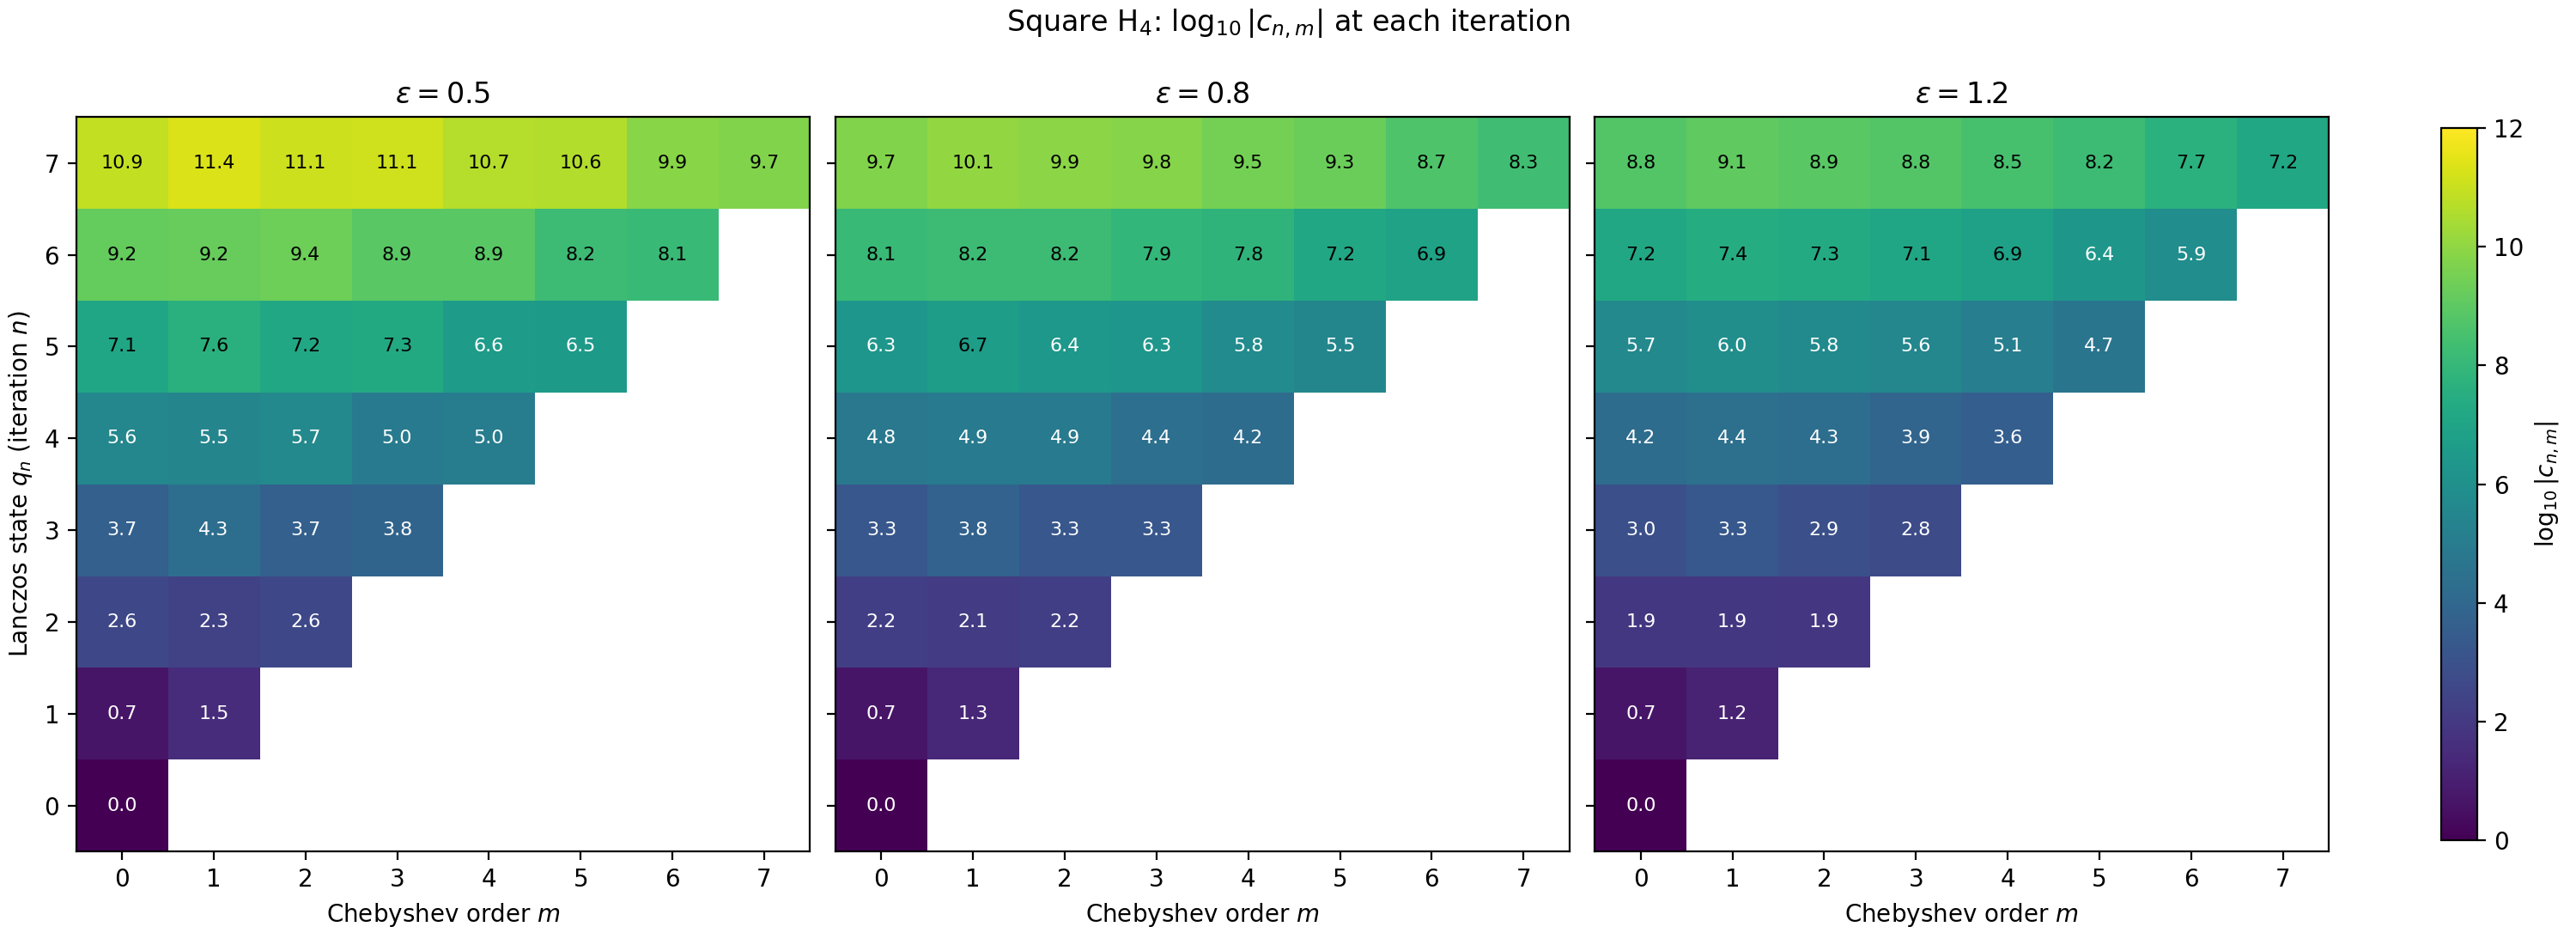
\includegraphics[width=0.90\linewidth]{output/ocqkudsin/chebyshev_coefficient_heatmap.png}
\end{center}
\vspace{-0.6em}
{\small\textbf{Heatmap reading:} each colored cell is
$\log_{10}|c_{n,m}|$; blank cells have $m>n$, so that coefficient does not
exist at that iteration.}

\end{document}
